 \documentclass[
	twoside,
	numbers=noenddot, 
	a4paper, 12pt,
	chapterprefix=true, appendixprefix=true,    % Kapitel 1 Einleitung oder 1 Einleitung 
	listof=totoc                                % Abbildungs/Tabellenverzeichnis
]{scrbook} 

%========================================================================================
% How-to-compile
% Compilation is the easiest and newest with xelatex:
%   1. Install inkscape and set path to inkscape folder (only for the svg-package)
%   2. Set command
%    xelatex.exe -shell-escape -synctex=1 -interaction=nonstopmode %.tex
%   3. Set default bibliography tool to "biber"
%
% Notes:
% 		- in theory you can remove "-shell-escape" as it is only used for the svg-package
%     - you could switch to pdflatex or lualtex, but you have to change the fontspec-package
%========================================================================================	

%========================================================================================
% Makros
%========================================================================================	
%========================================================================================
% Titel, Name
%========================================================================================
\newcommand{\tit}{{Signalverarbeitung f\"ur das Bewegungstracking von kinematischen Ketten}}
\newcommand{\subtit}{}
\newcommand{\ath}{Vorname Nachname}
\newcommand{\locdate}{Kiel, 2024}

%========================================================================================
% Mathe Formatierungen
%========================================================================================
\newcommand{\transp}{^\textrm{\footnotesize{T}}}                              % Transpose
\newcommand{\herm}{^\textrm{\footnotesize{H}}}                                % Hermitrian
\newcommand{\expect}[1]{\textrm{E}\left\{\,\displaystyle{{#1}}\,\right\}}     % Erwartungswert
\newcommand{\mse}[1]{\textrm{E}\left\{\left|{#1}(n)\right|^{2}\right\}}       % Mittlerer Qudratische Erwartungswert
\newcommand{\E}{\operatorname{E}}

\newcommand{\tindex}[1]{_{\textrm{\footnotesize{#1}}}}                        % Text tiefgestellt, nicht kursiv
\newcommand{\exponent}[1]{^{\textrm{\footnotesize{#1}}}}                      % Text tiefgestellt, nicht kursiv
\newcommand{\tindexTwo}[2]{_{\footnotesize{#1}\textrm{\footnotesize{#2}}}}    % Text tiefgestelt, erst kursiv, dann nicht kursiv
\newcommand{\subit}[1]{_{\mathit{#1}}}                                        % Text tiefgestellt, kursiv

\newcommand{\Exp}[1]{\mathrm{E}\!\left\{{#1}\right\}}                         % Ewartungswert
\newcommand{\ExpLeft}{\mathrm{E}\!\left\{\right\}}                            % Ewartungswert Klammer links
\newcommand{\ExpRight}{\mathrm{E}\!\right\}}                                  % Ewartungswert Klammer rechts
\newcommand{\ExpSmall}[1]{\mathrm{E}$\,$\!\{{#1}\}}                           % Ewartungswert, klein

\newcommand{\abs}[1]{\lvert {#1} \rvert}                                      % Betrag
\newcommand{\absSq}[1]{\abs{#1}\exponent{2}}                                  % Betragsquadrat
\newcommand{\norm}[1]{\lVert {#1} \rVert}                                     % Norm
\newcommand{\normSq}[1]{\norm{#1}\exponent{2}}                                % Quadratnorm
\newcommand{\Smo}[1]{\overline{#1}}                                           % Geglättete Variable
\newcommand{\SmoSq}[1]{\Smo{#1\exponent{2}}}                                  % Geglättetes Betragsquadrat
\newcommand{\unl}[1]{\underline{#1}}                                          % Variable unterstrichen
\newcommand{\round}[1]{\ensuremath\left\lfloor#1\right\rceil}                 % Runden einer Variable
\newcommand{\eExpOmega}{\big( e^{\footnotesize{\, j \Omega}} \big) }          % e hoch Omega
\newcommand{\freqMu}{\big( \mu \big) }

\newcommand{\vectorize}[1]{\textrm{VEC}\left\{\displaystyle{{#1}}\right\}}    % Vektorisieren
\newcommand{\diagonalize}[1]{\textrm{DIAG}\left\{\displaystyle{{#1}}\right\}} % Diagonaliseren

%========================================================================================
% Matrizen und Vektoren
%========================================================================================
\newcommand{\bvec}[1]{\mbox{\boldmath ${#1}$}}                 % Vektoren fett
\newcommand{\bmat}[1]{\mbox{\boldmath \underline{${#1}$}}}     % Matrizen fett, roman

%========================================================================================
% Misc commands
%========================================================================================
\newcommand{\red}[1]{\textcolor{red}{[#1]}}        % Notes and ToDos
\newcommand{\qm}[1]{``#1''}                        % Anführungszeichen
\newcommand{\engl}{engl.}                          % Englische abgekürzt
\newcommand{\OverSqrtHz}{/$\sqrt{\text{Hz}}$}      % Wurzel-Hertz

%========================================================================================
% General defines
%========================================================================================
\newcommand{\ffsAxes}{0.7}
\newcommand{\ffsLegend}{0.7}
\newcommand{\ffsNumbers}{0.7}
\newcommand{\ffsFormula}{0.7}
\newcommand{\ffsFormulaSFrac}{0.8}
\newcommand{\ffsExp}{0.5}	

%========================================================================================
% Legacy defines 
%========================================================================================
\newcommand{\tsup}[1]{^{\text{#1}}}
\newcommand{\tidx}[1]{_{\text{{#1}}}}

\newcommand{\argx}[1]{\ensuremath{\text{arg}\left\{#1\right\}}}
\newcommand{\absx}[1]{\ensuremath{\left|#1\right|}}
\newcommand{\absxnormal}[1]{\ensuremath{|#1|}}
\newcommand{\lgx}[1]{\ensuremath{\text{lg} \left( #1\right) }}
\newcommand{\maxx}[1]{\ensuremath{\text{max}\left\{#1\right\}}}
\newcommand{\minx}[1]{\ensuremath{\text{min}\left\{#1\right\}}}
\newcommand{\normx}[1]{\ensuremath{\left\|#1\right\|}}

%========================================================================================
% Abkürzungen
%========================================================================================
\newcommand{\AD}{AD}
\newcommand{\DA}{DA}

\newcommand{\EBASNR}{EBASNR}
\newcommand{\SNR}{$\text{SNR}$}
\newcommand{\DNR}{$\text{DNR}$}
\newcommand{\LOD}{$\text{LOD}$}

\newcommand{\MEMS}{MEMS}

\newcommand{\MVDR}{MVDR}

\newcommand{\NLMS}{NLMS}
\newcommand{\LMS}{LMS}
\newcommand{\AP}{AP}
\newcommand{\RLS}{RLS}

%========================================================================================
% Allgemeine Größen
%========================================================================================

%% Allgemein
\newcommand{\fs}{\ensuremath{f\tidx{s}}}

%% Indizes
\newcommand{\td}{\ensuremath{n}}	   % Digital time
\newcommand{\ta}{\ensuremath{t}}    % Analog time
\newcommand{\fb}{\ensuremath{\mu}}  % Frequency bin
\newcommand{\fri}{\ensuremath{k}}   % Frame index


%========================================================================================
% Custom Packages
%========================================================================================
\usepackage{tabu}
\usepackage{upgreek}
\usepackage{textgreek}
\usepackage{xfrac}
\usepackage{mathrsfs}
\usepackage{fontenc} % calls \usepackage[EU1]{fontenc}
\usepackage{lmodern}
\usepackage[ngerman]{babel}
\usepackage{amsmath}
\usepackage{amssymb}
\usepackage{bm}
\usepackage{blindtext}
\usepackage{cases}
%\usepackage[caption=false,font=footnotesize]{subfig}                                           % sfrac
\usepackage{color}
\usepackage[section]{placeins}        % nicht zu weit "floaten..."
\usepackage[
	hidelinks,
	pdftitle = {\tit - \subtit},
	pdfauthor = {\ath},
	bookmarks = true,
	bookmarksopen = true
	]{hyperref} 

\newlength{\figurewidth}
\usepackage{psfrag}
\usepackage[process=auto, cleanup={.tex,.dvi,.ps,.pdf,.log,.out, .bbl}]{pstool} % process=all -> render all psfrag replacements, auto all none
\usepackage{graphicx}
\usepackage{booktabs}
\usepackage{textgreek}

% Set folders for svg images
\usepackage[usetransparent=false]{svg}
\svgpath{{01_einleitung/images/}{02_grundlagen/images/}{03_konzept/images/}{04_simulationen/images/}{05_eval/images/}{06_ende/images/}{07_appendix/images/}}

% For including .tikz files
\usepackage{pgfplots}
\pgfplotsset{compat=newest,compat/show suggested version=false}
\usepackage{tikzscale}

\usepackage{tikz}
\usepackage{tikz-cd}
\usetikzlibrary{plotmarks}
\usetikzlibrary{arrows.meta}
\usetikzlibrary[patterns,shapes.arrows,external]
\usetikzlibrary{decorations.pathreplacing,calligraphy}
\usepackage{scalefnt}

% Externalization is to compile each plot as a separate TeX job
\usepgfplotslibrary{external}

\usepackage{csquotes}
\usepackage[maxnames = 1, maxbibnames = 15, backend=biber, style=alphabetic, backref=true, doi=false,isbn=false,url=false, bibencoding=ascii]{biblatex}% style=numeric
\addbibresource{literatur.bib}

\usepackage{epsfig}
\usepackage{xcolor,import}
%\usepackage{transparent}
\usepackage{tabularx}
\newcolumntype{Y}{>{\centering\arraybackslash}X}
\usepackage{multirow}
\usepackage{colortbl}

\usepackage[toc,nonumberlist,automake,nopostdot,style=listdotted]{glossaries}[=v4.46]%
\renewcommand*{\glsnamefont}[1]{\textmd{\textrm{#1}}}
\setlength{\glslistdottedwidth}{.3\linewidth}
%\setlength{\glsdescwidth}{0.8\linewidth}

%\usepackage[pass]{geometry}
\usepackage[top=25mm, bottom=35mm, left=25mm, right=25mm]{geometry} % offenbar default bei scrbook: top=25mm, bottom=35mm

\usepackage{scrwfile}
\usepackage{calc} 
\usepackage[Option]{overpic}
\usepackage{siunitx}
\usepackage{multicol}
\usepackage{array}
\usepackage{tabularx}
\usepackage{subcaption}
%\usepackage{subfigure}
\newcommand{\inputTikZ}[2]{%
     \scalebox{#1}{\input{#2}}}  
%========================================================================================
% Custom Glossar-Style
%========================================================================================
\newglossarystyle{altlistdotted}%
{%
   \glossarystyle{tree}%
   \renewcommand{\glossaryentryfield}[5]{%
     \hangindent0pt\relax
     \parindent0pt\relax
     \makebox[\glslistdottedwidth][l]%
     {%
       \glsentryitem{##1}\textbf{\glstarget{##1}{##2}}%
       \unskip\leaders\hbox to 2.1mm{\hss.}\hfill\strut
     }%
     \parbox[t]{\linewidth-\glslistdottedwidth}{##3}\par \vspace{0.5mm}}%
}
\setglossarystyle{altlistdotted} 

%========================================================================================
% Anlegen der Glossare
%========================================================================================
\newglossary[slg]{lat}{sls}{slo}{Verzeichnis lateinischer Symbole}
\newglossary[olg]{gre}{ols}{olo}{Verzeichnis griechischer Symbole}
\newglossary[alg]{abk}{als}{alo}{Abkürzungsverzeichnis}
\newglossary[plg]{notation}{pls}{plo}{Notation}
\makeglossaries

%========================================================================================
% Glossar und Farben
%========================================================================================
%========================================================================================
% Abkürzungen
%========================================================================================
\newglossaryentry{wE}{type=abk,sort={wE},name={w.E.},description={willkürliche Einheit}}
\newglossaryentry{Engl}{type=abk,sort={Engl},name={engl.},description={englisch}}

\newglossaryentry{AD}{type=abk,sort={AD},name={\AD},description={Analog-Digital}}
\newglossaryentry{DA}{type=abk,sort={DA},name={\DA},description={Digital-Analog}}

\newglossaryentry{EBASNR}{type=abk,sort={EBASNR},name={\EBASNR},description={geschätztes, biomagnetisches und gemitteltes \SNR{}  (\engl{}: \textit{Estimated Biomagnetic Averaged Signal-to-Noise Ratio})}}
\newglossaryentry{SNR}{type=abk,sort={SNR},name={\SNR},description={Signal-zu-Rausch-Verhältnis (\engl{}: \textit{Signal-to-Noise Ratio})}}
\newglossaryentry{DNR}{type=abk,sort={DNR},name={\DNR},description={Störungs-zu-Rausch-Verhältnis (\engl{}: \textit{Distortion-to-Noise Ratio})}}
\newglossaryentry{LOD}{type=abk,sort={LOD},name={\LOD},description={Detektionslimit (\engl{}: \textit{Limit of Detection})}}

\newglossaryentry{MEMS}{type=abk,sort={MEMS},name={\MEMS},description={mikro-elektromechanische Systeme (\engl{}: \textit{Microelectromechanical Systems})}}

\newglossaryentry{MVDR}{type=abk,sort={MVDR},name={\MVDR},description={Minimum Variance Distortionless Beamformer (\engl{}: \textit{Minimum Variance Distortionless Beamformer })}}

\newglossaryentry{NLMS}{type=abk,sort={NLMS},name={\NLMS{}-Algorithmus},description={normalisierter stochastischer Gradientenalgorithmus (\engl{}: \textit{Normalized Least Mean Square Algorithm})}}
\newglossaryentry{LMS}{type=abk,sort={LMS},name={\LMS{}-Algorithmus},description={stochastischer Gradientenalgorithmus (\engl{}: \textit{Least Mean Square Algorithm})}}
\newglossaryentry{AP}{type=abk,sort={AP},name={\AP},description={Affine Projektion (\engl{}: \textit{Affine Projection})}}
\newglossaryentry{RLS}{type=abk,sort={RLS},name={\RLS{}-Algorithmus},description={rekursives stochastisches Gradientenverfahren (\engl{}: \textit{Recursive Least Squares Algorithm})}}

\newglossaryentry{AlN}{type=abk,sort={AlN},name={AlN},description={Aliminiumnitrid}}
\newglossaryentry{FeCoSiB}{type=abk,sort={FeCoSiB},name={FeCoSiB},description={metallisches Glas (Eisen-Cobalt-Silizium-Bor)}}
\newglossaryentry{PZT}{type=abk,sort={PZT},name={PZT},description={Blei-Zirkonat-Titanat}}
\newglossaryentry{Au}{type=abk,sort={Au},name={Au},description={Gold}}
\newglossaryentry{Cr}{type=abk,sort={Cr},name={Cr},description={Chrom}}
\newglossaryentry{Cu}{type=abk,sort={Cu},name={Cu},description={Kupfer}}
\newglossaryentry{Ta}{type=abk,sort={Ta},name={Ta},description={Tantal}}
\newglossaryentry{MnIr}{type=abk,sort={MnIr},name={MnIr},description={Mangan-Iridium}}

%========================================================================================
% Notation
%========================================================================================
\newglossaryentry{nE}{type=notation,sort={g},name={$\E{x(n)}$},description={Erwartungswert von $x(n)$} }

\newglossaryentry{nvec}{type=notation,sort={a},name={\ensuremath{\bvec{x}}},description={Vektor (fettgedruckt, klein)} }
\newglossaryentry{nmat}{type=notation,sort={a},name={$\bvec{X}$},description={Matrix (fettgedruckt, groß)} }
\newglossaryentry{nskalar}{type=notation,sort={a},name={$x$},description={Skalar, zumeist zeitabhängig (nicht fettgedruckt, klein)} }
\newglossaryentry{nSkalar}{type=notation,sort={a},name={$X$},description={Skalar, zumeist frequenzabhängig (nicht fettgedruckt, groß)} }

\newglossaryentry{nj}{type=notation,sort={b},name={$j$},description={imaginäre Einheit, $j^2=-1$} }
\newglossaryentry{njRe}{type=notation,sort={b},name={$\Re{\left\{ z \right\} }$},description={Realteil der komplexen Zahl $z$} }
\newglossaryentry{njIm}{type=notation,sort={b},name={$\Im{\left\{ z \right\} }$},description={Imaginärteil der komplexen Zahl $z$} }
\newglossaryentry{njAbs}{type=notation,sort={b},name={$\absx{z}$},description={Betrag der komplexen Zahl $z$} }
\newglossaryentry{njArg}{type=notation,sort={b},name={$\argx{z}$},description={Argument der komplexen Zahl $z$} }
\newglossaryentry{njKonj}{type=notation,sort={b},name={$z^{*}$},description={konjugierte komplexe Zahl zur komplexen Zahl $z$} }

\newglossaryentry{nbvecTransp}{type=notation,sort={c},name={$\bvec{x}\transp{}, \bvec{X}\transp{}$},description={transponierter Vektor/Matrix} }
\newglossaryentry{nbvecHerm}{type=notation,sort={c},name={$\bvec{x}\herm{}, \bvec{X}\herm{}$},description={hermitischer Vektor/Matrix, $ \bvec{X}\herm{} = \left(\bvec{X}^{*} \right)\transp{}$} }

\newglossaryentry{nlog10}{type=notation,sort={d},name={$\lgx{z}$},description={Logarithmus der reellen Zahl $z$ zur Basis 10} }

\newglossaryentry{nhadamard}{type=notation,sort={e},name={$\bvec{x} \circ \bvec{y}$},description={Hadamard-Produkt, elementweise Multiplikation} }

\newglossaryentry{nnorm}{type=notation,sort={e},name={$\normx{\bvec{x}}$},description={Norm des Vektors} }

%\newglossaryentry{nDFT}{type=notation,sort={f},name={$\DFTmath{}\left\{ \cdot{} \right\}$},description={\DFT{} der Ordnung \Ndft{}} }
%\newglossaryentry{nDSTFT}{type=notation,sort={f},name={$\DSTFTmath{}\left\{ \cdot{} \right\}$},description={\DSTFT{} der Ordnung \Ndft{}} }


\newglossaryentry{nmax}{type=notation,sort={h},name={$\maxx{x(n)}$},description={Maximum von $x(n)$} }
\newglossaryentry{nmin}{type=notation,sort={h},name={$\minx{x(n)}$},description={Minimum von $x(n)$} }

%========================================================================================
% Symbols
%========================================================================================
%% Indizes
\newglossaryentry{td}{type=lat,sort={na},name={\td},description={Zeitindex}  }
\newglossaryentry{ta}{type=lat,sort={ta},name={\ta},description={Zeit}  }
\newglossaryentry{fb}{type=gre,sort={mau},name={\fb},description={Frequenzstützstelle}  }
\newglossaryentry{fri}{type=lat,sort={ka},name={\fri},description={Blockindex}  }

\newglossaryentry{fs}{type=lat,sort={fas},name={\fs},description={Abtastrate}  }



%========================================================================================
% Ende
%========================================================================================
\glsaddall

%-------------------------------------------------------------------------
% Color palette definition
%-------------------------------------------------------------------------
\xdefinecolor{colparula8darkblue}{RGB}{  53,42,135}
\xdefinecolor{colparula8blue}{RGB}{  2,104,225}
\xdefinecolor{colparula8darktuerkis}{RGB}{ 16,142,210}
\xdefinecolor{colparula8tuerkis}{RGB}{  15,174,185}
\xdefinecolor{colparula8green}{RGB}{  101,190,134}
\xdefinecolor{colparula8darkoragene}{RGB}{ 192,188,96}
\xdefinecolor{colparula8oragene}{RGB}{  255,195,55}
\xdefinecolor{colparula8yellow}{RGB}{  249,251,14}

\xdefinecolor{colgreen1}{RGB}{  200,255,200}
\xdefinecolor{colgreen2}{RGB}{  150,255,150}
\xdefinecolor{colgreen3}{RGB}{  100,255,100}

\xdefinecolor{colred1}{RGB}{  255,200,200}
\xdefinecolor{colred2}{RGB}{  255,100,100}
\xdefinecolor{colneutral}{RGB}{  255,255,255}

\xdefinecolor{colgray}{RGB}{  220,220,220}

\xdefinecolor{backgroundcolor}{RGB}{  255,255,255}
 

%========================================================================================
% Titel und Autor
%========================================================================================
\title{\tit}
\subtitle{\subtit}
\author{\ath}

%========================================================================================
% Setzen von custom Größen
%========================================================================================
\renewcommand{\floatpagefraction}{.6}% vorher: .5 
\renewcommand{\textfraction}{.15} % vorher: .2 
\renewcommand{\topfraction}{.85}     % vorher: .7 
\renewcommand{\bottomfraction}{.5}  % vorher: .3 
\setcounter{topnumber}{3} % vorher: 2 
\setcounter{bottomnumber}{1} % vorher: 1 
\setcounter{totalnumber}{5} % vorher: 3
\renewcommand{\dbltopfraction}{.8} % vorher: .7 
\renewcommand{\dblfloatpagefraction}{.6}% vorher: .5 

% Begin des Dokuments
\begin{document}

   \pagenumbering{roman}
   
   %========================================================================================
   % Trennung von bestimmten Wörtern
   %========================================================================================
   \hyphenation{Sig-nal}
   \hyphenation{Sig-na-le}
   \hyphenation{Nutz-sig-nal-kom-po-nen-te}
   
   %========================================================================================
   % Titelseite
   %========================================================================================
   %-------------------------------------------------------------------------
% Titelseite
%-------------------------------------------------------------------------
\begin{titlepage}
   \centering
   \LARGE
   \vspace*{10mm}
   
   {
      \textbf{\tit{}}\\[0.5ex]
      \subtit{}
   }
   		
   \vspace{2cm}
   \textbf{Dissertation}

   \vspace{2ex}
   {\Large
      zur Erlangung des akademischen Grades \\[0.5ex]
      Doktor der Ingenieurwissenschaften \\[0.5ex]
      (Dr.-Ing.) \\[0.5ex]
      der Technischen Fakultät \\[0.5ex]
      der Christian-Albrechts-Universität zu Kiel \\[0.5ex]
   }

   \vspace{2.8cm}
   {
   	\Large
   	vorgelegt von 
   }\\[2ex]
   \textbf{
   	Tobias Schmidt
   }

   \vspace{2.5cm}
	\locdate
\end{titlepage}

\newpage

%-------------------------------------------------------------------------
% Titelrückseite
%-------------------------------------------------------------------------
\thispagestyle{empty}
\quad
\vspace{25mm}

\vfill
\begin{tabbing}
   Tag der Einreichung: \hspace{16ex} \= \red{XX.XX.2024?} \\
   Tag der Disputation: \> \red{XX.XX.2024?} \\ \\
	Berichterstatter: \>  Prof.~Dr.-Ing.~Gerhard Schmidt \\
	 \>  \red{Prof.~Dr.~rer.~nat.~XXX} \\
	 \>   \red{Prof.~Dr.-Ing.~Dr.-Ing.~habil.~XXX} \\
\end{tabbing}

 
   \newpage
   
   %========================================================================================
   % Erklärung (Einbinden, wenn eingereicht wird)
   %========================================================================================
   \chapter*{Erklärung}
%\addcontentsline{toc}{chapter}{Erklärung}

\vspace{3cm}
Hiermit erkläre ich, dass die vorliegende Dissertation nach Inhalt und Form meine eigene Arbeit ist und von mir selbst verfasst worden ist, wobei mir mein Doktorvater Herr Prof. Dr.-Ing. Gerhard Schmidt beratend zur Seite stand. Die Arbeit war weder in Teilen noch im Ganzen Bestandteil eines früheren Prüfungsverfahrens und ist an keiner anderen Stelle zur Prüfung eingereicht. Der Inhalt der Arbeit wurde in Teilen in meinen wissenschaftlichen Publikationen veröffentlicht. Dies ist in der Arbeit entsprechend vermerkt. Die Arbeit ist nach bestem Wissen und Gewissen konform mit den Regeln guter wissenschaftlicher Praxis, welche durch die Deutsche Forschungsgemeinschaft festgelegt sind.  
\vspace{3cm}

\noindent\rule{0.75\textwidth}{.5pt}\\
\mbox{\quad \ \ \ \ Ort} \hspace{2cm} Datum \hspace{2cm} \ath{}\\
   \cleardoubleevenpage
   
   %========================================================================================
   % Danksagung (Einbinden, wenn wirklich veröffentlicht wird)
   %========================================================================================
   %\chapter*{Danksagung}
%\addcontentsline{toc}{chapter}{Erklärung}

\vspace{3cm}

Danke
   %\cleardoubleevenpage
   
   %========================================================================================
   % Kurzfassung und Abstract
   %========================================================================================
   \chapter*{Kurzzusammenfassung}

   TEXT

\chapter*{Abstract}

   TEXT

   
   %========================================================================================
   % Inhaltsverzeichnis, Abbildungsverzeichnis, Tabellenverzeichnis
   %========================================================================================
   \pdfbookmark[0]{Inhaltsverzeichnis}{toc}
   \tableofcontents 
   \listoffigures
   \listoftables
   
   %========================================================================================
   % Abkürzungen, Notation und Symbole
   %========================================================================================
   \printglossary[type=abk]
   \printglossary[type=notation]
   
   \chapter*{Symbolverzeichnisse}
   \addcontentsline{toc}{chapter}{Symbolverzeichnisse}
   
   \setglossarysection{section}
   \printglossary[type=lat]
   \printglossary[type=gre]
    
   %========================================================================================
   % Einleitung
   %========================================================================================
   \chapter{Einleitung}
\label{chap:01_einleitung}
\pagenumbering{arabic}

   Text

   \section{Motivation}
   \label{sec:01_motivation}
   
      Text
      
   \section{Einordnung der Arbeit}
   \label{sec:01_einordnung}
      
      Text
      
   \section{Aufbau der Arbeit}
   \label{sec:01_aufbau}
   
      Text
   
   %========================================================================================
   % Grundlagen
   %========================================================================================
   \chapter{Bewegunsanalyse}
\label{chap:Bewegungsanalyse}
\section{Bewegungsbeschreibung}
\label{sec:anatomy}
\subsection{Gelenkarten}
Kugelgelenke
Sattelgelenke
Eigelenke
Scharniergelenke
\subsection{Bewegungsdefinition}

\section{Konventionelle Systeme}
\subsection{optische Systeme}
\subsection{IMU basierte Systeme}

\section{Schlussbetrachtung}



      
      
   
   %========================================================================================
   % Konzept
   %========================================================================================
   \chapter{Magnetische Räumliche Signalmerkmale}
\label{chap:raeumliches_merkmal} 
Ziel dieser Arbeit ist es, Orientierungen von kinematischen Elementen und der Positionen zu schätzen. Die Orientierungen lassen sich mit räumlichen Vektoren beschreiben. Die Merkmale für die Signalverarbeitung sollen sich daran orientieren. In diesem Kapitel werden zunächst Verfahren beschrieben mit denen magnetische Felder analytisch beschrieben werden können. Daraus abgeleitet wird ein räumliches Signalverarbeitungsmerkmal eingeführt und die Zusammenhänge zwischen Position, Orientierung und diesem Merkmal vorgestellt und diskutiert.

\section{Modellierung magnetischer Felder}

\subsection{Biot-Savart}

Theoretische
Elektrotechnik
Marco Leone
Elektromagnetische Feldtheorie für
Ingenieure
- kurze Beschreibung wie mit Biot-Savart magnetische Felder beschrieben werden, nur für einen Stromfaden 

Bild von Biot Savart

\subsection{Magnetischer Dipol}
Nolting
Grundkurs
Theoretische Physik 3

Bild Dipol Berechnung
\subsubsection{Herleitung des Dipolfeldes}

\subsubsection{Bestimmung des Dipolmoment}
\subsubsection{Betrag des Magnetfeldes}

\subsection{Quasistationäre Felder}
Nolting
Grundkurs
Theoretische Physik 3

\section{3D Spule}
Bild und Simulationsbild
Wieso ist das gut? Lokalisierungsansätze mit 3D- Sensoren \dots

In dieser Arbeit wird eine 3D-Spule zur Anregung künstlicher Magnetfelder verwendet. 3D-Spule sind 3 ineinander verschachtelte Spulen. Jede einzelne hat ihre Öffnung in eine unterschiedliche Richtung, und die Normalenvektoren dieser Flächen stehen senkrecht zueinander. Damit stehen auch die resultierenden Dipolmomente senkrecht zueinander und diese drei Dipolmomente spannen ein Koordinatensystem auf. In Abbildung \ref{fig:3DCoil} ist eine kleine 3D-Spule und das zugehörige Simulationsobjekt dargestellt. 

\begin{figure}
    \centering
    \subfloat[Simulation Object]{
        \inputTikZ{0.6}{03_raeumliches_merkmal/images/3DCoil.tikz}
        \label{fig:Sim3D}
    }
    \subfloat[3D coil]{
        \begin{overpic}[width=0.5\textwidth,trim = 0 0 0 0]{03_raeumliches_merkmal/images/Real_3D_Coil_with_legend.pdf}
            \put(10,10){3\,cm}
            %\put(2,25){3\,cm}
        \end{overpic}
        \label{fig:Real3D}
    }
    \caption{3D-Spule: \subref{fig:Sim3D} skizziert das modellierte Simulationsobjekt. Ein Foto der entsprechenden Realisierung ist in \subref{fig:Real3D} zu sehen. Beide Objekte bestehen aus drei zueinander orthogonal stehenden Spulen. Die rote Spule steht für die X-Spule, die grüne für die Y-Spule und die blaue für die Z-Spule. Somit  }
    \label{fig:3DCoil}
\end{figure}

Die Spule kann unterschiedlich angesteuert werden. Zum einen gibt es die Möglichkeit, die drei Spulen einzeln anzusteuern und diese auf Sensorseite wieder voneinander zu trennen. Zum anderen können die drei Dipole so angesteuert werden, sodass durch Überlagerung ein resultierender Dipol in beliebiger Richtung erzeugt werden kann. Die zweite Ansteuerung wird in dieser Arbeit verwendet.

\section{Sensormodellierung}
In diesem Kapitel werden Zusammenhänge zwischen magnetischen Aktuatoren und magnetischen Sensoren hergeleitet. Um die Herleitung möglichst einfach zu halten wird der Sensor als ideal angenommen. „Ideal“ bedeutet, dass der Sensor in einem einzigen Punkt lokalisiert ist und dass die Ausgabe des Sensors eine ungestörte Projektion des Dipolfeldes auf die Hauptsensorachse ist. Der Ausgang $B\tindex{sensor}(\vec{r},\vec{e}\tindex{s})$ ergibt sich dann als

\begin{equation}
    B\tindex{sensor}(\vec{r},\vec{e}_s) =  \vec{B}\tindex{dip}(\vec{r}) \cdot \vec{e}_s.
    \label{eq:Sensorprojektion}
 \end{equation}

\section{Maximalvektor}
\label{sec:maximum_vector}
Der Maximalvektor ist ein Signalmerkmal, das verwendet werden kann, wenn 3D-Aktuatoren und 1D-Sensoren verwendet werden. Dabei sei angenommen, dass der Aktuator im Ursprung und der Sensor am Ort $\vec{r}$ mit der Sensorachse $\vec{e}\tindex{s}$ lokalisiert ist. Der Maximalvektor beschreibt die Polarisierungsrichtung des magnetischen Dipols in welcher das Sensorausgangssignal maximal wird.

\subsection{Lokalisierungszusammenhänge}
\label{subsec:Lokalisierungszusammenhänge}
    \subsubsection{Orientierung und normierte Position}
Im Folgenden soll der Zusammenhang zwischen dem Maximalvektor (MV) $\vec{e}\tindex{max}$, dem normierten Positionsvektor $\vec{e}\tindex{r}$ und der Sensororientierung $\vec{e}\tindex{s}$ hergeleitet werden. 

Da ein Zusammenhang zwischen den einzelnen normierten Vektoren gesucht wird, nutzen wir eine normierte Beschreibung des Dipolfeldes und kommen zu folgender Beschreibung

\begin{equation}
    \vec{B}\tindex{norm} = \frac{4 \pi r^3}{ m } \vec{B}\tindex{dip}(\vec{r}) =  3\vec{e}_r(\vec{e}_\text{m}\cdot\vec{e}_r)-\vec{e}_\text{m}.
    \label{eq:magDipNorm}
\end{equation}


\begin{figure}[h!]
    \centering
    \begin{overpic}[width=0.7\textwidth,trim = 0 0 0 0]{04_lokalisierung/images/Angledescription.pdf}
        \put(82,44){$\phi\tindex{s}$}
        \put(62,25){$\phi$}
        \put(20,14){$\phi\tindex{m}$}
        \put(6,30){$\theta\tindex{m}$}
        \put(13,26){$\vec{m}$}
        \put(90,5){$x$}
        \put(57,60){$y$}
        \put(2,62){$z$}
        \put(40,30){$\vec{r}$}
        \put(75,47){$\vec{e}\tindex{s}$}
    \end{overpic}
    \caption{
    Verwendetes Setup für die Herleitung: $\vec{e}\tindex{r}$ und $\vec{e}\tindex{s}$ liegen beide in der $xy$-Ebene. $\phi\tindex{m}$ und $\theta\tindex{m}$ definieren die Richtung des rotierenden magnetischen Dipols $\vec{e}\tindex{m}$ in Kugelkoordinaten.}
    \label{fig:Winkelbeschreibung}
\end{figure}

Für die Herleitung werden zunächst einige Annahmen getroffen. Zwei nicht kolineare Vektoren spannen immer eine Ebene auf. Daher kann das Koordinatensystem so gelegt werden, dass $\vec{e}\tindex{r}$ und $\vec{e}\tindex{s}$ in der $xy$-Ebene liegen. Die beiden Vektoren seien daher wie folgt definiert.
\begin{equation}
    \vec{e}_r = \left[\begin{array}{c} \cos(\phi)\\ \sin(\phi) \\ 0\end{array}\right] \quad \textrm{and} \quad
    \vec{e}_s = \left[\begin{array}{c} \cos(\phi\tindex{s})\\ \sin(\phi\tindex{s}) \\ 0\end{array}\right].
    \label{eq:defErEs}
\end{equation}
Die dreidimensionale magnetische Quelle hat ein konstantes magnetisches Dipolmoment der Stärke $m$ die jedoch in jede beliebige Richtung zeigen kann. Die Definition der Richtung ist an die Rücktransformation von Kugelkoordinaten in kartesische Koordinaten angelehnt. Das Dipolmoment ist in kartesischen Koordinaten definiert wie folgt
\begin{equation}
    \vec{e}_m = \left[\begin{array}{c} \cos(\phi\tindex{m})\sin(\theta\tindex{m})\\ \sin(\phi\tindex{m})\sin(\theta\tindex{m}) \\ \cos(\theta\tindex{m}) \end{array}\right].
    \label{eq:defEm}
 \end{equation}
Durch einsetzen der Vektordefinition in Gl. \ref{eq:magDipNorm} kommt man zu den folgenden vektoriellen Komponenten des Dipolfeldes

 \begin{eqnarray}
    B\tindex{norm,x}(\phi,\phi\tindex{m},\theta\tindex{m})&=&\big[3\cos(\phi)^2-1\big]\,\cos(\phi\tindex{m})\,\sin(\theta\tindex{m}) \nonumber \\ &+&  3 \,\sin(\phi\tindex{m})\,\sin(\theta\tindex{m})\,\sin(\phi)\,\cos(\phi),
    \label{eq:magNormX} \\[2mm]
    B\tindex{norm,y}(\phi,\phi\tindex{m},\theta\tindex{m})&=&\big[3\sin(\phi)^2-1\big]\,\sin(\phi\tindex{m})\,\sin(\theta\tindex{m}) \nonumber\\ &+& 3 \,\cos(\phi\tindex{m})\,\sin(\theta\tindex{m})\,\cos(\phi)\,\sin(\phi),
    \label{eq:magNormY} \\[2mm]
    B\tindex{norm,z}(\theta\tindex{m}) &=& - \cos(\theta\tindex{m}).
    \label{eq:magNormZ}
\end{eqnarray}
Mit Gl. \ref{eq:magDipSensor} kommt man zum Sensorsignal $B\tindex{sensor}$

\begin{equation}
    B\tindex{sensor}(\phi,\phi\tindex{s},\phi\tindex{m},\theta\tindex{m},r) =  \frac{ m }{4 \pi r^3} \big((\cos(\phi\tindex{s})\, B\tindex{norm,x}(\phi,\phi\tindex{m},\theta\tindex{m}) + \sin(\phi\tindex{s})\, B\tindex{norm,y}(\phi,\phi\tindex{m},\theta\tindex{m})\big).
    \label{eq:normSensor}
\end{equation}

Bezüglich einer Varierung von $\theta\tindex{m}$, wird das Sensorsignal maximal wenn $\theta\tindex{m} = \frac{\pi}{2}$. Dies zeigt außerdem, dass die Komponente des rotierenden Dipols, die senkrecht zur von $\vec{e}\tindex{r}$ und $\vec{e}\tindex{s}$ aaufgespannten Ebene liegt, keinen Einfluss auf das Sensorsignal hat. Diese Beobachtung zeigt, dass der MV in dieser aufgespannten Ebene liegen muss. Diese Erkenntnis vereinfacht die Problemstellung zu einem 2D-Problem und kann daher in einer Ebene weiter betrachtet werden.

Um einen Zusammenhang zwischen den drei Vektoren zu erhalten wird nun angenommen, dass der Sensor auf $x$-Achse lokalisiert sei. Die Vektoren sind in kartesischen Koordinaten wie folgt definiert

\begin{equation}
    \vec{e}_r = \left[\begin{array}{c} 1\\ 0 \end{array}\right],\qquad
    \vec{e}_m = \left[\begin{array}{c} \cos(\phi\tindex{m}) \\ \sin(\phi\tindex{m}) \end{array}\right],\qquad
    \vec{e}_s = \left[\begin{array}{c} \cos(\phi\tindex{s})\\ \sin(\phi\tindex{s})\end{array}\right].
    \label{eq:defErEmEs}
\end{equation}
Dies führt zum folgenden magnetischen normierten Feld für die einzelnen Komponenten $B\tindex{norm,x},B\tindex{norm,y},B\tindex{norm,z}$ führt 

\begin{eqnarray}
    B\tindex{norm,x}(\phi) &=& 2  \cos(\phi\tindex{m}),
    \label{eq:magNorm2DX}\\
    B\tindex{norm,y}(\phi) &=& - \sin(\phi\tindex{m}),
    \label{eq:magNorm2DY}\\
    B\tindex{norm,z}(\phi) &=& 0.
    \label{eq:magNorm2DZ}\\
\end{eqnarray}
Die Projektion auf die Sensorachse führt zu:
\begin{equation}
    B\tindex{sensor}(\phi\tindex{s},\phi\tindex{m})= \frac{ m }{4 \pi r^3} \big( 2  \cos(\phi\tindex{m})  \cos(\phi\tindex{s}) - \sin(\phi\tindex{m})  \sin(\phi\tindex{s}) \big).
    \label{eq:formel12}
\end{equation}
Es wird der Wert $\phi\tindex{max}$ von $\phi\tindex{m}$ gesucht, für den $B\tindex{sensor}$ maximal wird. Dafür wird Gleichung \ref{eq:formel12} nach $\phi\tindex{m}$ differenziert und man erhält einen Zusammenhang zwischen $\phi\tindex{max}$ und $\phi\tindex{s}$.
\begin{equation}
    \frac{\text{d}B_\text{sensor}(\phi\tindex{m})}{d\phi\tindex{m}}=\frac{ m }{4 \pi r^3}\left ( -2 \sin(\phi\tindex{m})\cos(\phi\tindex{s})-\sin(\phi\tindex{s})  \cos(\phi\tindex{m})\right )
    \label{eq:formel13}
\end{equation}

\begin{equation}
    -2 \sin(\phi\tindex{max})\cos(\phi\tindex{s})-\sin(\phi\tindex{s})  \cos(\phi\tindex{max}) = 0.
\end{equation}
\begin{equation}
    -2\cdot\tan(\phi\tindex{max})= \tan(\phi\tindex{s}).
    \label{eq:relMaxS}
\end{equation}
    
    Gleichung \ref{eq:relMaxS} zeigt einen Zusammenhang zwischen $\vec{e}\tindex{max}$,$\vec{e}\tindex{r}$ und $\vec{e}\tindex{s}$. Dieser Zusammenhang gilt nicht nur für $\phi = 0$ sondern gilt auch wenn der Sensor nicht auf der $x$-Achse lokalisiert sind. In Abbildung \ref{fig:maxvectorAcngles} ist diese Veralgemeinerung gezeigt. 
    
    \begin{figure}[h!]
\centering
\begin{overpic}[width=1\textwidth,trim = 0 0 0 0]{04_lokalisierung/images/MaxvectorAngles.pdf}
    \put(75,24){$\phi\tindex{s}$}
    \put(78,20.5){$\phi\tindex{max}$}
    \put(90,2){$x$}
    \put(44,2){$x$}
    \put(48,20){$y$}
    \put(0,20){$y$}
    \put(20,2){$\vec{r}$}
    \put(55,10){$\vec{r}$}
    \put(69,22){$\vec{e}\tindex{s}$}
    \put(30,10){$\vec{e}\tindex{s}$}
    \put(33,7){$\phi\tindex{s}$}
    \put(37,2.5){$\phi\tindex{max}$}
    \put(63,8){$\phi$}
    \put(5,2){3D-Spule}
    \put(50,2){3D-Spule}
    \put(20,6){Sensor}
    \put(63,18){Sensor}
    \put(75,16){$\vec{e}\tindex{max}$}
    \put(28,1){$\vec{e}\tindex{max}$}
\end{overpic}
\caption{ Die Beziehung in Gleichung\,\ref{eq:formel14} ist unabhängig vom Winkel $\phi$. Außerdem wird die eindeutige Beziehung zwischen den 3 Einheitsvektoren $\vec{e}_s, \vec{e}_{max},$ und $\vec{e}_r$ gezeigt.}
\label{fig:maxvectorAcngles}
\end{figure}
    
    Dieser kann genutzt werden um bei bekanntem $\vec{e}\tindex{r}$ und detektiertem Maximalvektor $\vec{e}\tindex{max}$ das zugehörige $\vec{e}\tindex{s}$ zu bestimmen. Die zugehörige Berechnungsvorschrift wird im folgenden einmal gezeigt. Hinzufügen Verallgemeinerung Formel relmaxs


\begin{enumerate}

    \item Zunächst wird die Rotationsachse bestimmt $\vec{e}_\text{n}$:
    %
    \begin{equation}
        \vec{e}_n = \frac{\vec{e}\tindex{max} \times \vec{e}_r }{\|\vec{e}\tindex{max} \times \vec{e}_r\|}.
        \label{eq:formel15}
    \end{equation}
    
    \item Im zweiten Schritt wird der Winkel zwischen MV und dem normierten Positionsvektor bestimmt:
    %
    \begin{equation}
        \phi\tindex{max} = \arccos(\vec{e}\tindex{max} \cdot \vec{e}_r).
        \label{eq:formel16}
    \end{equation}
    
    \item Anschließend wird der Winkel zwischen dem Ortseinheitsvektor und der Sensorausrichtung aus Gl. \ref{eq:relMaxS}:
    %
    \begin{equation}
        \phi\tindex{s} = \arctan\big(-2\tan(\phi\tindex{max})\big).
        \label{eq:formel17}
    \end{equation}
    
    \item  Abschließend kann für jeden $\vec e_r$ die Sensororientierung $\vec e_\text{s}$ wie folgt berechnet werden:
    %m
    \begin{equation}
        \vec{e}_\text{s} = \cos(\phi\tindex{s})(\vec{e}_n \times \vec{e}_r)\times \vec{e}_n + \sin(\phi\tindex{s}) (\vec{e}_n \times\vec{e}_r).
        \label{eq:formel18}
    \end{equation}
    \end{enumerate}

    Daraus ergibt sich, dass mit dem MV für jede relative Position eine Sensororientierung bestimmt werden kann. Die Verteilung der möglichen Positions- Orientierungspaare sind in Abbildung \ref{fig:PotentialPoses} dargestellt.
    
    \begin{figure}[h]
        \centering
        \inputTikZ{0.5}{04_lokalisierung/images/potentialposes.tikz}
        \caption{ Blaue Vektoren: Berechnete Sensorausrichtungen $\vec e_s$ für verschiedene Werte der Sensorposition $\vec r$. Der Startpunkt jedes blauen Vektors entspricht dem entsprechenden $\vec r$. Gelber Vektor: Der maximale Vektor im Ursprung, immer in $y$-Richtung polarisiert. Beachten Sie, dass die Längen der blauen Vektoren hier nicht von Interesse sind, da nur die Richtungen relevant sind.}
        \label{fig:PotentialPoses}
    \end{figure} 

	\subsubsection{Distanz zwischen Sensor und Quelle}
        Die Ausrichtung eines Einheitsvektors lässt sich mit 2 Winkeln beschreiben und enthält daher zwei Informationen. Mit einer 3D-Spule lassen sich wie im Grundlagenkapitel gezeigt, drei orthogonale Signale erzeugen aus denen sich dann drei Informationen extrahieren lassen. Als dritte Information definieren wir die Länge $A$ des Maximalvektors. Diese ist in den Grundlagen als Betrag eines 3D-Spulenfeldes eingeführt worden. Der Sensor misst eine gewichtete Überlagerung der drei Spulensignale. Die Gewichtung erfolgt über die in den Grundlagen beschriebenen Übertragungsfaktoren. Mit den einzelnen Übertragungsfaktoren $G\tindex{x}(\vec{r}),G\tindex{y}(\vec{r}),G\tindex{z}(\vec{r})$ und den Spulensignalen lässt sich das Signal am Sensor wie folgt beschreiben:
        \begin{equation}
            B\tindex{sensor}(t,\vec{r}) = G\tindex{x}(\vec{r}) S\tindex{x}(t) +G\tindex{y}(\vec{r}) S\tindex{y}(t) + G\tindex{z}(\vec{r}) S\tindex{z}(t).
            \label{eq:GewSensSignal}
        \end{equation}
        Hier muss nochmal nachgearbeitet werden.
        
        Definition der Intensität, Zusammenhang zwischen Intensität und Distanz, Zusammenhang zwischen normierter Position und Distanz.

        Der Sensor misst eine gewichtete Summe $B\tindex{sensor}$ der drei Spulensignale $S\tindex{x}t),S\tindex{y}(t),S\tindex{z}(t)$. Die Gewichtung der einzelnen Signale wird durch die Dipolnäherung beschrieben $G\tindex{x}(\vec{r}),G\tindex{y}(\vec{r}),G\tindex{z}(\vec{r})$
 


      %========================================================================================
   % Konzept
   %========================================================================================
   \chapter{Lokalisierungsalgorithmen}
\label{chap:char_localization}
Im Folgenden Kapitel soll die verwendete Algorithmik vorgestellt werden. Dabei wird zunächst ein magnetisch räumliches Signalverarbeitungsmerkmal vorgestellt. Dieses Merkmal wird für eine relative Lokalisierung (Rekonstruktion der einer kinematischen Kette) und eine absolute Lokalisierung innerhalb eines definierten Arbeitsraums genutzt. In diesem Kapitel werden die Sensoren als ideal angenommen, um die algorithmische Herleitung nicht unnötig kompliziert zu machen. 

Es wurde ein iterativer Algorithmus entwickelt, der Vorwissen über die Anatomie integriert und so effizient die Haltung schätzt. Die Prämisse für den Algorithmus ist, dass jedes kinematische Element, mit Ausnahme des ersten, mit einem Magnetfeldsensor ausgestattet wird. Am ersten kinematischen Element ist eine 3D-Spule befestigt. Desweiteren wird zunächst angenommen, dass die Sensorachse diesselbe Orientierung wie das zugehörige kinematische Element und der Sensor genau in der Mitte des kinematischen Elements lokalisiert. Im Allgemeinen hat die Pose eines Sensors fünf Freiheitsgrade, drei für die Position, sowie 2 für die Orientierung der Sensorachse. Durch die Kopplung des Sensors an die Elemente wird die Anzahl der Freiheitsgrade reduziert zur Anzahl der Freiheitsgrade des Gelenks.

Absolute Lokalisierung

\section{Simulationsetup}
Die Herleitung des Algorithmus soll mit kleinen Simulationen veranschaulicht werden. Die Simulation besteht aus drei idealen Dipolquellen, die die verwendete Quelle modellieren, sowie zunächst einem ideal angenommenen Punktsensor. Dies bedeutet, dass der Sensor die Projektion des magnetischen Feldes auf die sensitive Achse des Sensors detektiert. Im späteren Verlauf wird für die Herleitung des Schätzalgorithmus eine kinematische Kette mit bis zu zwei Elementen verwendet. Eine solche Kette ist in Abbildung \ref{fig:Sensorplacement}.

\begin{figure}[h!]
		\centering
		\begin{overpic}[width=\textwidth,trim = 0 0 0 0]{04_lokalisierung/images/Sensorplacement.png}
			\put(0,48){3D-Spule}
			\put(27,27){$\vec{r}\tindex{j1}$}
			\put(59,53){$\vec{r}\tindex{j2}$}
			\put(40,47){$l\tindex{js1}$}
			\put(62,25){$l\tindex{js2}$}
			\put(38,32){Sensor 1}
			\put(59,38){Sensor 2}
		\end{overpic}
		\caption{Sensor- und Quellenanordnung: Die kinematische Kette besteht aus zylinderförmigen Element, sowie Gelenken die diese verbinden und die Möglichkeit haben diese zu bewegen. Die linke Seite zeigt die Anordnung der Quellen und Sensoren auf der kinematischen Kette. Auf dem ersten Element ist eine 3D-Spule angebracht. Die weiteren Elemente sind mit Sensoren ausgerüstet. Diese sind auf der Mittelachse des kinematischen Elements (siehe rechter Teil).
		}
		\label{fig:Sensorplacement}
	\end{figure}

\section{Maximalvektor}
	In der vorgestellten Algorithmik wird ein räumliches Feature eingeführt. Der Hauptgedanke dahinter ist, dass eine kinematische Kette durch die Ausrichtung der einzelnen Elemente beschrieben werden können. Die Ausrichtung der einzelnen Elemente kann in kartesischen Koordinaten mit einem Vektor der Länge 1 beschrieben werden. Die Zielgröße ist dementsprechend eine Anzahl an räumlichen 3D-Vektoren, daher wurde als Eingangsgröße ebenfalls ein räumlicher Vektor ausgewählt.
	Der Maximalvektor (MV) wird wie folgt definiert. Es sei eine dreidimensionale Quelle $\vec{m} = \left[\begin{array}{c} m\tindex{x}\\ m\tindex{y} \\ m\tindex{z}\end{array}\right] $, lokalisiert im Koordinatenursprung, sowie ein Sensor am Ort $\vec{r}$ mit einer Orientierung der sensitiven Achse $\vec{e}_\text{s}$. 
	Ein magnetischer Dipol sei definiert wie folgt [Zitat]
	\begin{equation}
		\vec{B}\tindex{dip}(\vec{r},\vec{m}) = \frac{1}{4\pi r^2}\frac{3\vec{r}(\vec{m}\cdot\vec{r})-\vec{m}r^2}{r^3}.
		\label{eq:magDipolDef}
	\end{equation}
	Ein idealer Sensor misst die Projektion des magnetischen Feldes auf die Sensorachse
	\begin{equation}
		B\tindex{sensor}(\vec{r},\vec{e}_s,\vec{m}) =  \vec{B}\tindex{dip}(\vec{r}) \cdot \vec{e}_s.
		\label{eq:magDipSensor}
	 \end{equation}
	Der MV ist in diesem Fall, die Dipolorientierung $\frac{\vec{m}}{|\vec{m}|}$ für die $B\tindex{sensor}(\vec{r},\vec{e}_s,\vec{m})$ maximal wird.


        
        
\section{Relative Lokalisierung}
In diesem Kapitel wird ein Ansatz aufbauend auf den theoretischen Grundlagen des vorherigen Kapitels vorgestellt. Zunächst wird ein iterativer Ansatz gezeigt, mit dem die Haltung einer kinematischen Kette effizient geschätzt werden kann. Desweiteren werden die Eindeutigkeit, Optimierungen (des Modells und des Rechenbedarfs) und eine Nachverarbeitung vorgestellt. 


\subsection{Iterativer Algorithmus}

    Der Algorithmus kombiniert die magnetischen Zusammenhänge und das Vorwissen über die Anatomie. Die Prämisse des Algorithmus ist, dass bei korrekt angenommener Sensororientierung, mit der Anatomie die korrekte Position des Sensors berechnet werden kann. Mit der korrekten Position kann mithilfe der magnetischen Zusammenhänge die korrekte Sensororientierung bestimmt werden. Diese Selbstkonsistenz wird nun ausgenutzt.

    Für den Algorithmus werden die Position des Gelenks $\vec{r}\tindex{j}$ und die Distanz zwischen Gelenk und Sensor benötigt. Es wird zunächst eine zufällige Orientierung $\vec{\hat{e}}\tindex{s,1}$ des Sensors angenommen. Mit der Anatomie wird die zugehörige Sensorposition bestimmt

    \begin{equation}
        \vec{\hat{r}}\tindex{s,$i$} = \vec{r}\tindex{j} + l\tindex{js} \, \vec{\hat{e}}\tindex{s,$i$} .
        \label{eq:formelIter1}
    \end{equation}
    
    Im nächsten Schritt wird die Sensororientierung für die Position mit den magnetischen Zusammenhängen, die in den Gleichungen \,\ref{eq:formel15} bis \ref{eq:formel18} beschrieben wurden, bestimmt.

    \begin{equation}
        	\vec{\hat{e}}\tindex{s,$i+$1} = \vec{f}(\vec{\hat{r}}\tindex{s,$i$},\vec{e}\tindex{max}).
        \label{eq:formelIter2}
    \end{equation} 
    
    Diese Porzedur wird mit der jeweils neuen Orientierung wiederholt bis die Veränderung der Orientierung einen Schwellwert unterschreitet. Der Ablauf des Algorithmus ist in Abbildung \ref{fig:Flussdiagramm} zu sehen.
    

\begin{figure}[h]
    \centering
    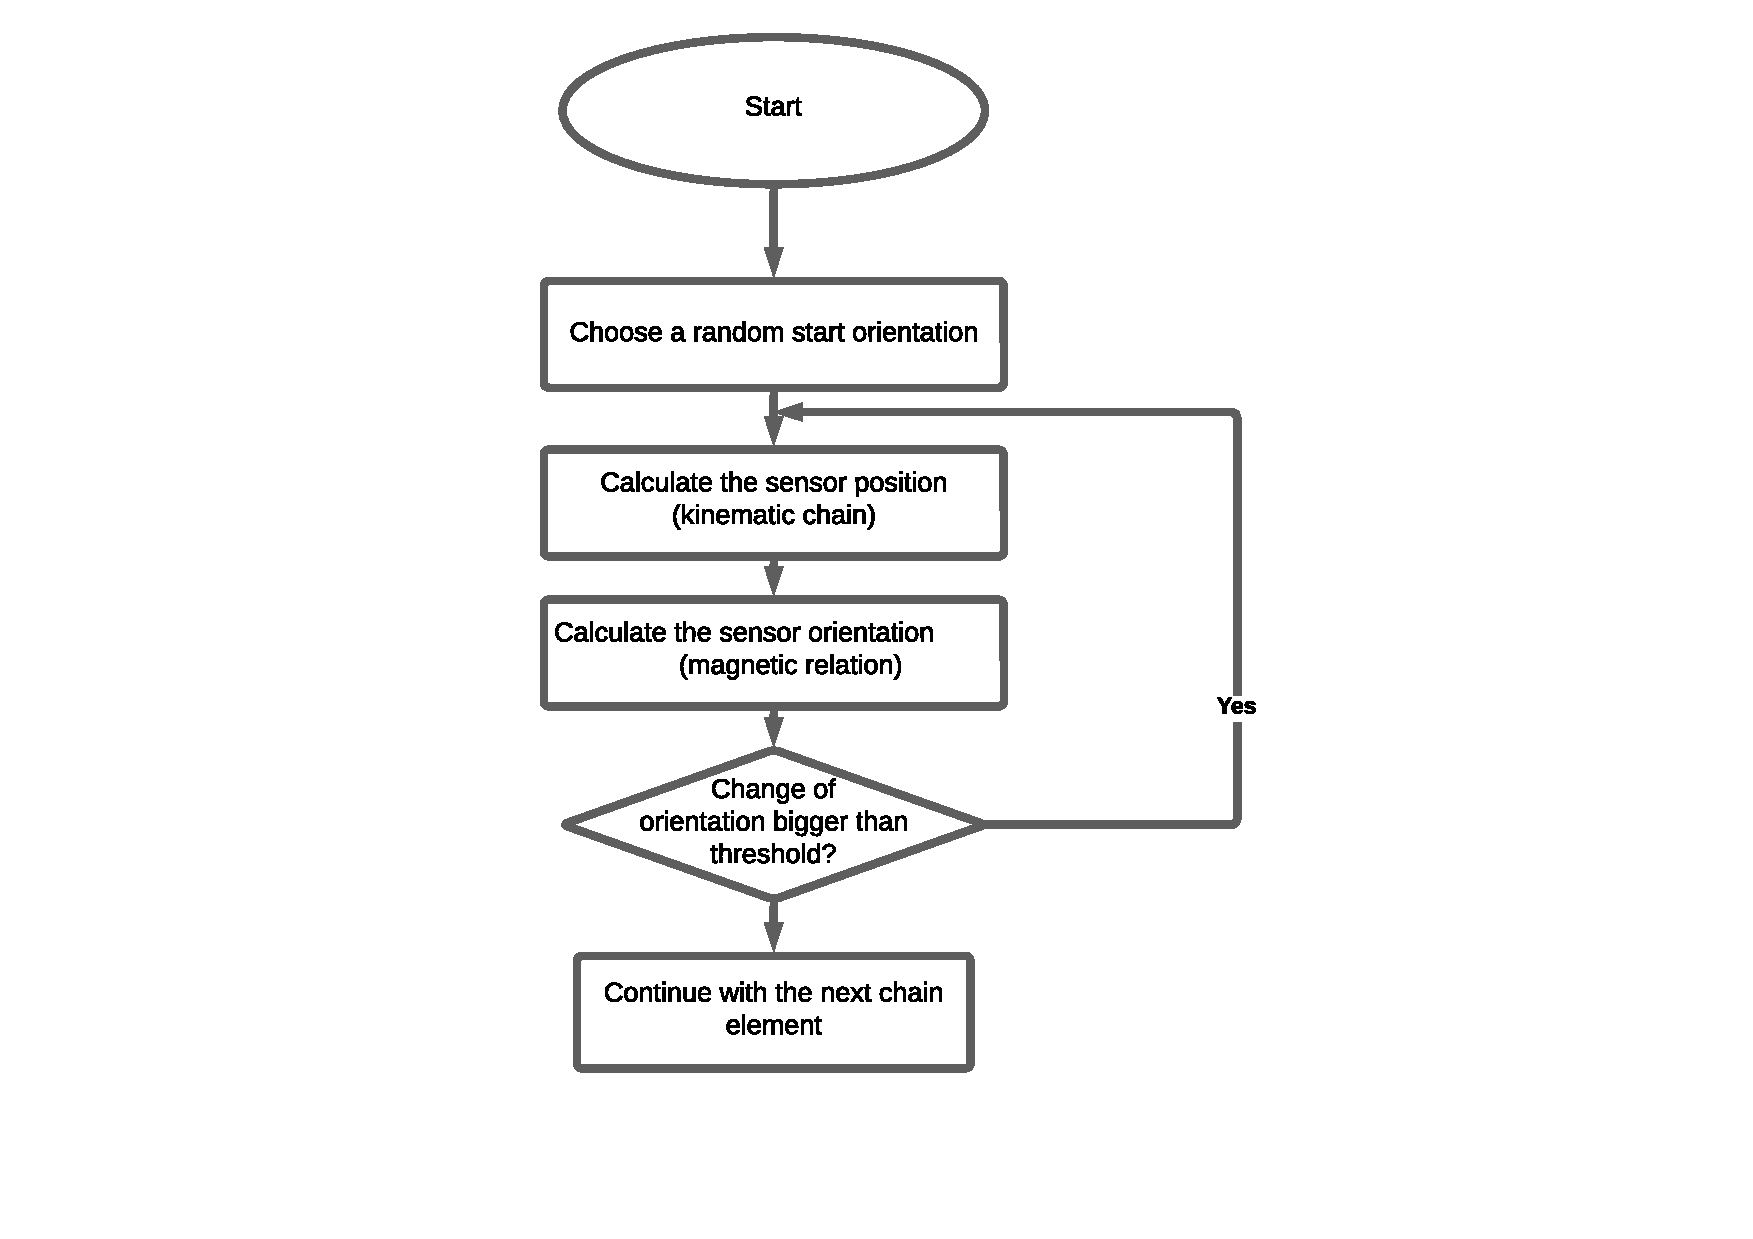
\includegraphics[width=0.5\textwidth,trim = 0 0 0 0]{04_lokalisierung/images/Flussdiagramm.pdf} 
    \caption{Flussdiagramm des iterativen Algorithmus: Der Algorithmus startet mit einer zufällig ausgewählten Sensororientierung. Im ersten Schritt wird die relative Sensorposition bestimmt. Daraus wird die zugehörige Sensororientierung bestimmt. Diese Prozedur wird wiederholt, bis die Veränderung zwischen den Iterationen kleiner ist als ein definierter Schwellenwert und Konvergenz erreicht ist. Diese Orientierung ist dann die geschätzte Lösung.}
    \label{fig:Flussdiagramm}
\end{figure}

	Eine Visualisierung dieser Prozedur ist in Abbildung, wo die Orientierungen und Positionen für die einzelnen Iterationen dargestellt ist. Nach etwa 15 Iterationen stimmt die Sensorpose mit einer potentiellen Pose überein.

\begin{figure}[h]
    \centering
    
    \inputTikZ{0.35}{04_lokalisierung/images/legend.tikz} 
    \label{fig:legend}
    \subfloat[Setup]{
        \begin{overpic}[scale=0.17,trim= 4cm 0 4cm 0]{04_lokalisierung/images/PotentialPoses_for_Inkscape_Setup_grid.png}
            \put(50,45){$x$}
            \put(30,65){$y$}
            \label{fig:Setup}
        \end{overpic}
    }
    \subfloat[Iteration 1]{
        \begin{overpic}[scale=0.17,trim= 4cm 0 4cm 0]{04_lokalisierung/images/PotentialPoses_for_Inkscape_Iteration1_grid.png}
            \label{fig:Iteration1}
        \end{overpic}
    }
    \subfloat[Iteration 2]{
        \begin{overpic}[scale=0.17,trim= 4cm 0 4cm 0]{04_lokalisierung/images/PotentialPoses_for_Inkscape_Iteration2_grid.png}
            \label{fig:Iteration2}
        \end{overpic}
    }
    \subfloat[Iteration 15]{
        \begin{overpic}[scale=0.17,trim= 4cm 0 4cm 0]{04_lokalisierung/images/PotentialPoses_for_Inkscape_Iteration4_grid.png}
            \label{fig:Iteration15}
        \end{overpic}
    }
    \caption{Beispielhafter iterativer Prozess: Diese Abbildung zeigt die Iterationen für einen einfachen Aufbau. Die Unterabbildung \ref{fig:Setup} zeigt den verwendeten Aufbau mit dem Koordinatensystem. Der Ursprung dieses Aufbaus befindet sich am ersten kinematischen Kettenelement, wo sich auch die Quelle befindet. Die Quelle ist mit dem ersten kinematischen Element so verbunden, dass die relative Position der Quelle zur kinematischen Kette immer konstant ist. In den folgenden Abbildungen wurde das Koordinatensystem weggelassen. Die blauen Vektoren stellen die möglichen Posen für die erkannte MV dar. Die hellgrüne Konstruktion zeigt die Bodenwahrheit. Der rote Vektor ist ein normalisierter Positionsvektor des Sensors, der auf die potentielle Pose in dieser Richtung zeigt. Der Sensor ist am zweiten Knochen angebracht. Er wird durch ein schwarzes Rechteck mit einem Vektor in die sensitive Richtung dargestellt. Unterabbildung\,\subref{fig:Iteration1} beginnt mit einer Knochenorientierung in $x$-Richtung. Für einige Iterationen sind die kinematische Kette und der zugehörige Positionsvektor dargestellt. Nach 15 Iterationen (sub-figure\,\subref{fig:Iteration15}) stimmt die Sensorpose mit einer potentiellen Pose (ground truth) überein und der Algorithmus konvergiert.}
    \label{fig:Concept_Algorithm}
\end{figure}

Einfluss der Längenänderungen auf die Konvergenzgeschwindigkeit
Q einfügen

\subsection{Eindeutigkeit der Lösung}
	Im folgenden wird die die Eindeutigkeit des vorgestellten iterativen Algorithmus geprüft. Der Algorithmus ist eindeutig, wenn jedem möglichen Eingangsvektor $\vec{e}\tindex{max}$ eine Sensororientierung $\vec{e}\tindex{s}$ zu geordnet werden kann. Die Eingangs- und Ausgangsvektoren werden dafür in jeweils zwei Winkel aufgeteilt. 

    Der Eingangsvektor besitzt zwei Freiheitsgrade, die die Richtung definieren. Die Orientierung des Sensors wird ebenfalls über zwei Winkel (Freiheitsgrade) definiert. Im folgenden wird zunächst eine Entkopplung der Ein- und Ausgangsvektoren vorgenommen, also hat eine Eingangsgröße nur Einfluss auf eine Ausgangsgröße. Da es sich auf beiden Seiten um Winkel handelt, müssen diesen Winkeln Rotationsachsen zugeordnet werden. 

    Zunächst wird der Zusammenhang aus Kapitel \ref{subsec:Lokalisierungszusammenhänge}, dass $\vec{e}_{max}$, $\vec{e}_s$ und $\vec{e}_r$ in einer Ebene liegen verwendet. Dies bedeutet gleichzeitig auch, dass die Gelenkspostion $\vec{r}_j$ in dieser Ebene liegen muss. Dies ist der Fall, da diese von der Sensorposition in Richtung der Sensororientierung liegt. Daher kann der normalen Vektor $\vec{e}_{n}$ dieser Ebene wie folgt bestimmt werden
    \begin{equation}
        \vec{e}_{n} = \frac{\vec{e}_{max}\times \vec{r}_j}{|\vec{e}_{max}\times \vec{r}_j|}
    \end{equation}

    Dies bedeutet, dass die Sensororientierung auf einer Ebene, einer Ebenschar die durch $\vec{r}_j$ definiert wird. Daher ist die erste Rotationsachse $\frac{\vec{r}_j}{|\vec{r}_j|}$. Die erste Eingangsgröße $\phi_{m,1}$ ist daher der Winkel zwischen $\vec{e}_n$ und einer frei wählbaren Bezugsachse. Die Bezugsachse muss nur senkrecht zu $\vec{r}_j$ stehen. Die Ausgangsgröße $\phi_{s,1}$ entspricht dann der Eingangsgröße.  Dieser Zusammenhang ist in Abbildung \ref{fig:Visualisierung_Uniqueness_Ebene} zu sehen.
    
	\begin{figure}[h!]
		\centering
		\begin{overpic}[width=0.7\textwidth,trim = 0 0 0 0]{04_lokalisierung/images/Visualisierung_Uniqueness_gedreht.pdf}
			\put(82,44){$\phi\tindex{s}$}
			\put(62,25){$\phi$}
			\put(20,14){$\phi\tindex{m}$}
			\put(6,30){$\theta\tindex{m}$}
			\put(13,26){$\vec{m}$}
			\put(90,5){$x$}
			\put(57,60){$y$}
			\put(2,62){$z$}
			\put(40,30){$\vec{r}$}
			\put(75,47){$\vec{e}\tindex{s}$}
		\end{overpic}
		\caption{ Beschreibung des ersten Freiheitsgrades: In der Abbildung ist eine kinematische Kette, bestehend aus zwei Elementen. Im Ursprung ist eine 3D-Spule an der die kinematische Kette angebracht ist. In gelb ist $\vec{e}_{max}$ dargestellt. Dieser spannt gemeinsam mit $\vec{r}_j$ die gelbe Ebene auf. Auf dem zweiten Kettenelement ist ein Sensor in der Mitte des Sensors angebracht und das Gelenk ist so geknickt, dass der Sensor leicht nach unten schaut. Die $XY$-Ebene ist in grau dargestellt. In der Abbildung ist gut zu sehen, dass die gelbe Ebene, durch das erste und zweite ELement schneidet. Es ist erkennbar, dass sowohl $\vec{r}_j$, $\vec{r}_s$ und $\vec{e}_s$ in dieser Ebene liegen.
			}
		\label{fig:Visualisierung_Uniqueness_Ebene}
	\end{figure}
Die Lösung ist nun auf einen Freiheitsgrad eingeschränkt. Der zweite Freiheitsgrad, ist nun der Winkel der um den Normalenvektor dreht. Als Bezugsachse wird im Folgenden ein $\vec{r}_j$ verwendet. Die Eingangsgröße ist dann der Winkel $\phi_{m,2}$ zwischen $\vec{e}_{max}$ und $\vec{r}_j$ und die Ausgangsgröße $\phi_{s,2}$ ist der Winkel zwischen $\vec{e}_s$ und $\vec{r}_j$.
	\begin{figure}[h!]
		\centering
		\begin{overpic}[width=0.7\textwidth,trim = 0 0 0 0]{04_lokalisierung/images/Eindeutigkeit_Ebene.pdf}
			\put(82,44){$\phi\tindex{s}$}
			\put(62,25){$\phi$}
			\put(20,14){$\phi\tindex{m}$}
			\put(6,30){$\theta\tindex{m}$}
			\put(13,26){$\vec{m}$}
			\put(90,5){$x$}
			\put(57,60){$y$}
			\put(2,62){$z$}
			\put(40,30){$\vec{r}$}
			\put(75,47){$\vec{e}\tindex{s}$}
		\end{overpic}
		\caption{
			Winkelzusammenhang: Die Abbildung zeigt den Ebenenschnitt, der gelben Ebene, von Abbildung \ref{fig:Visualisierung_Uniqueness_Ebene}. In der Abbildung ist die kinematische Kette in der von $\vec{e}_{max}$ und $\vec{r}_j$ aufgespannten Ebene. In gelb ist die zweite Eingangsgröße $\phi_{m,2}$ dargestellt. Der blaue Winkel zeigt die Ausgangsgröße $\phi_{s,2}$.
			}
		\label{fig:Visualisierung_Winkelbeschreibung_2}
	\end{figure}

Im Folgenden wird zunächst ein funktionaler Zusammenhang $\phi\tindex{max,2} = f(\phi\tindex{s,2})$ aufgestellt. Zu nächst sei die Gelenksposition $\vec{r}\tindex{j}$ wie folgt definiert, wobei $l\tindex{aj}$, der Distanz von Quelle zu Gelenk entspricht und auf 1 normiert wird um den Zusammenhang später verallgemeinern zu können.  
	\begin{equation}
		\vec{r}\tindex{j} = \left[\begin{array}{c} 1\\ 0 \end{array}\right] 
	\end{equation}
	Die Position des Sensors $\vec{r}\tindex{s}$ kann mit der Länge zwischen Sensor und Gelenk $l\tindex{js}$ wie folgt beschrieben werden.
	\begin{equation}
		\vec{r}\tindex{s} = \left[\begin{array}{c} 1+Q\cos(\phi\tindex{s,2})\\ Q\sin(\phi\tindex{s,2}) \end{array}\right] 
	\end{equation}
	Nun wird zunächst die Winkel zwischen $x$-Achse und $\vec{r}\tindex{s}$ bestimmt.
	\begin{equation}
		\phi\tindex{r} = \arctan\big(\frac{Q\cos(\phi\tindex{s,2})}{1+Q\sin(\phi\tindex{s,2})}\big)
	\end{equation}
	mit Gleichung \ref{eq:relMaxS} kann nun $\phi\tindex{max,2}$ bestimmt werden 
	\begin{equation}
		\phi\tindex{max,2} = -\arctan(\frac{1}{2} \tan(\phi\tindex{s,2} - \phi\tindex{r} ).
        \label{eq:uniqness_Value_2}
	\end{equation}
	
	
\begin{figure}
	\begin{subfigure}{0.5\textwidth}
	\scalefont{4}
		\centering
		\inputTikZ{0.225}{04_lokalisierung/images/q0_05_Unique.tikz}
		\caption{$0<Q<=0.5$}
		\label{fig:0_05_Unique}
	\end{subfigure}
	\hspace{0.25cm}
	\begin{subfigure}{0.5\textwidth}
	\scalefont{4}
		\centering
		\inputTikZ{0.225}{04_lokalisierung/images/q05_10_Unique.tikz}
		\caption{$0.5<Q<=1$}
		\label{fig:05_10_unique}
	\end{subfigure}
	\begin{subfigure}{0.5\textwidth}
	\scalefont{4}
		\centering
		\inputTikZ{0.225}{04_lokalisierung/images/q11_16_Unique.tikz}
		\caption{$1<Q$}
		\label{fig:bigger1_unique}
	\end{subfigure}
	\caption{ Funktionaler Winkelzusammenhang: In der Abbildung ist der Zusammenhang zwischen $\phi\tindex{s,2}$ und $\phi\tindex{max,2}$ für verschiedene Wertebereiche von $Q$. Die Abbildungen \ref{fig:0_05_Unique} und \ref{fig:bigger1_unique} zeigen eine eindeutige Zuordnung zwischen $\phi\tindex{s,2}$ und $\phi\tindex{max,2}$. In diesem Bereich gibt es für jeden Eingangsvektor einen zugehörigen Ausgangsvektor. In Abbildung \ref{fig:05_10_unique} ist der Zusammenhang für $0.5 < Q < 1$ zu sehen. Hier ist teilweise einem Wert für $\phi\tindex{max,2}$ zwei unterschiedliche Werte für $\phi\tindex{s,2}$ zugeordnet.}

    
	\label{fig:uniqueness}
\end{figure}

Dieser Zusammenhang ist nicht trivial und nicht einfach umkehrbar. In einem Skript wurde mit einer Auflösung von $1°$ Verläufe für Gleichung \ref{eq:uniqness_Value_2} für unterschiedliche $Q$ bestimmt. Die Ergebnisse sind in Abbildung \ref{fig:uniqueness} dargestellt. Aus der Abbildung geht hervor, dass der Algorithmus eindeutige Ergebnisse für $Q<=0.5$ und $Q>1$ liefert. In der späteren Anwendung muss dies beachtet werden, wobei bei einer SensorGlove Anwendung die kinematischen Elemente relativ klein ist. Dies führt zu einem kleinen $l\tindex{js}$ und somit zu einem kleinerem $Q$. 

\subsection{Analyse der benötigten Rechenleistung}
Analyse mit einer Matlabsimulation

\subsection{Optimierungen}
    Laufzeitoptimierung(LookUpTable), Korrektur von Modellfehlern (Dicke des Fingers, Verdrehung des Sensors)
    Diskussion...
	\subsection{Analyse der Unsicherheiten}
		Einführung virtuelle/mechanische Achsen,        

	\section{Absolute Lokalisierung}
		\subsection{Grundsätzliche Gedanken}
		\subsection{Ebenenschnitt}
		\subsection{Orientierung}
		

	

   
   %========================================================================================
   % Simulationen
   %========================================================================================
   \chapter{Umsetzung}
\label{chap:umsetzung}

  \section{Allgemeines zum Kapitel}
  \label{sec:allgemeines}  
  \section{Hardware}
	\section{Implementierung}

  \section{Diskussion}
  \label{sec:diskussion}
     
         
      
   
   %=================================== =====================================================
   % Evaluierung 
   %========================================================================================
   \chapter{Evaluierung}
\label{chap:Messergebnisse}

   
\section{Messszenarios}
\label{sec:eval_szenarios}


\section{Messergebnisse}
\label{sec:eval_ergebnisse}

\section{Fehlerdiskussion}
\label{sec:Fehlerdiskussion}



   
   %========================================================================================
   % Zusammenfassung und Ausblick
   %========================================================================================
   \chapter{Zusammenfassung und Ausblick}
\label{chap:ende_zusammenfassung_ausblick}

   Text

   \section{Zusammenfassung}
   \label{sec:ende_zusammenfassung}
   
      Text

   \section{Ausblick}
   \label{sec:ende_ausblick}
   
      Text
   
   %========================================================================================
   % Literaturverzeichnis
   %========================================================================================
   \printbibheading[title={Literaturverzeichnis},heading=bibintoc]%bibnumbered]
   \printbibliography[title={Publikationen mit Eigenbeteiligung},heading=subbibintoc,keyword=own]%subbibnumbered,subbibliography
   \printbibliography[title={Weitere Literatur}, heading=subbibintoc, notkeyword=own]
   
   %========================================================================================
   % Anhänge
   %========================================================================================
   \appendix
   \chapter{Weitere Messdaten}
\label{chap:appendix_a}
\pagenumbering{Roman}

   \section{Tmp}
   \label{sec:app_a_tmp}
   
      Text

      
   \chapter{Herleitung XXX}
\label{chap:appendix_b}

   Text

   \section{Tmp}
   \label{sec:app_b_tmp}
   
      Text

   
   %========================================================================================
   % Deprecated
   %========================================================================================
   %\chapter*{Erklärung}
%\addcontentsline{toc}{chapter}{Erklärung}

\vspace{3cm}
Hiermit erkläre ich, dass die vorliegende Dissertation nach Inhalt und Form meine eigene Arbeit ist und von mir selbst verfasst worden ist, wobei mir mein Doktorvater Herr Prof. Dr.-Ing. Gerhard Schmidt beratend zur Seite stand. Die Arbeit war weder in Teilen noch im Ganzen Bestandteil eines früheren Prüfungsverfahrens und ist an keiner anderen Stelle zur Prüfung eingereicht. Der Inhalt der Arbeit wurde in Teilen in meinen wissenschaftlichen Publikationen veröffentlicht. Dies ist in der Arbeit entsprechend vermerkt. Die Arbeit ist nach bestem Wissen und Gewissen konform mit den Regeln guter wissenschaftlicher Praxis, welche durch die Deutsche Forschungsgemeinschaft festgelegt sind.  
\vspace{3cm}

\noindent\rule{0.75\textwidth}{.5pt}\\
\mbox{\quad \ \ \ \ Ort} \hspace{2cm} Datum \hspace{2cm} \ath{}\\
   %\input{00_support/shaker_reihe}

\end{document}